\documentclass[journal,twocolumn]{IEEEtran}

\usepackage{enumitem}
\usepackage{hyperref}
\usepackage{caption}
\usepackage{graphicx}
\usepackage{float}
\usepackage{listings}
\usepackage{xcolor}   % Import xcolor for custom colors

\lstdefinelanguage{JavaScript}{
  keywords={typeof, new, true, false, catch, function, return, null, catch, switch, var, if, in, while, do, else, case, break},
  keywordstyle=\color{blue}\bfseries,
  ndkeywords={class, export, boolean, throw, implements, import, this},
  ndkeywordstyle=\color{darkgray}\bfseries,
  identifierstyle=\color{black},
  sensitive=false,
  comment=[l]{//},
  morecomment=[s]{/*}{*/},
  commentstyle=\color{purple}\ttfamily,
  stringstyle=\color{red}\ttfamily,
  morestring=[b]',
  morestring=[b]"
}

\lstset{
   language=JavaScript,
   backgroundcolor=\color{lightgray},
   extendedchars=true,
   basicstyle=\footnotesize\ttfamily,
   showstringspaces=false,
   showspaces=false,
   numbers=left,
   numberstyle=\footnotesize,
   numbersep=9pt,
   tabsize=2,
   breaklines=true,
   showtabs=false,
   captionpos=b
}

\title{Evaluating Software Using Black-Box and User Testing}

\author{\IEEEauthorblockN{Oliver Levay, Kristina Sedelius, Adam Tegelberg, Emma Haggren}
\\
\IEEEauthorblockA{\textit{Lunds tekniska högskola} \\
\textit{Lund University}\\
Lund, Sweden \\
(ol1662le-s, kr0363se-s, ad3444te-s, em5261ha-s)@student.lu.se}
}

\begin{document}
\maketitle
\IEEEpeerreviewmaketitle

\begin{abstract}
    This research project compares automated testing, using the software \textit{Cypress}, and manual human testing. This was done by creating three versions of a simple login page as an application and creating a quality assurance checklist relating to the quality attributes described in ISO/IEC 9126. The different versions each had a random set of faults related to the quality attribute requirements that were supposed to be fulfilled according to the quality assurance checklist. After creating the website, tests were written in Cypress using the checklist. The developers that created the website and that wrote the tests had very limited communication to ensure that the tests were not influenced by the implementation. Four tests subjects used the checklist to identify issues with the login page. Automatic testing was more reliable than human testing, a computer will not get tired or have opinions about what is worth testing. The human test subjects produced feedback that was never even considered by the research team. Automated tests written in Cypress might not have this ability. The results of the testing showed that the automated tests were more accurate and consistent. Furthermore, the results suggest that a combination of automated tests and human user testing in order to get the best of both worlds with the current tooling available. Evaluating if the detailed feedback that the human test subjects gave is a unique human trait was outside the scope of this paper. The team was surprised by how well automated testing could find faults in usability, and frustrated how hard it was to write automated usability tests.
\end{abstract}

\section{Introduction}
\subsection{Background}
Software quality assurance is crucial to ensure that applications meet user expectations and standards. This project focuses on evaluating a simple login page against the ISO/IEC 9126 product quality standards, which include the attributes functionality, reliability, usability, efficiency, maintainability and portability \cite{ISO}.

\subsection{Objective}
The goal of this research project is to compare automated Black-Box testing with human testing. The automated tests were written in Cypress and both the automated tests and the human tests were guided by a quality assurance checklist. We aim to answer the following research questions:
\begin{enumerate}
    \item What is the overlap between the software quality issues that can be identified by human testers and those that can be identified by automated Black-Box testing? %($A \cap B$)
    \item Which types of software quality problems can only be found by human testers, and which can only be identified by automated Black-Box testing? %($A \setminus B$ and $B \setminus A$)
    \item Which types of issues can't be identified by either method? %($A \cup B)^c$
\end{enumerate}

\section{Method}
\subsection{A login page}
A login page was chosen because of these main reasons.

\begin{enumerate}
    \item It's very common on the web, which means that all users have preexisting conceptions of how it should work.
    \item It's not too complicated to make.
    \item It's very important that it works as the user would expect, and that it works well, or the user will not be able to even try the product or service. The team believes that if the login page does not work all other type of testing is irrelevant. This makes the login page the most important part of a web-based business
\end{enumerate}
\subsection{Software Implementation}
Multiple versions of a simple login page was created using React. The versions were created with intentional issues connected to the ISO/IEC 9126 standards. At first a simple and functioning login page was created, then five new versions were created. Each initial version had a unique focus on exclusively functionality, reliability, usability, efficiency or portability. The introduced issues were:

\textbf{Functionality}:
\begin{itemize}
    \item Faulty logic for login-check, for example not requiring a password, or only being able to log in with admin and no other users.
    \item Password is not case-sensitive.
    \item Enter key disabled for logging in.
\end{itemize}

\textbf{Reliability}:
\begin{itemize}
    \item A pop-up when the login failed, that was irremovable preventing recoverability.
    \item A ten percent probability of randomly failing.
\end{itemize}

\textbf{Usability}:
\begin{itemize}
    \item Non-centered components.
    \item Text with small size, Comic Sans font, and low contrast from background color.
    \item Password- and username-field were switched.
    \item Cursor disappears when hovering over the login button.
    \item Overall visually displeasing.
\end{itemize}

\textbf{Efficiency}:
\begin{itemize}
    \item A delay caused by extremely inefficient search algorithm.
    \item Multiple confirm pop-ups before attempting a login.
\end{itemize}

\textbf{Portability}:
\begin{itemize}
    \item Unable to login on Firefox, Safari and Edge. Only usable with chrome.
\end{itemize}

Maintainability was excluded because it cannot be evaluated with either Cypress or user testing, as it requires analysis of the internal structure of the code. The team that are supposed to write the test cases, and the human test subjects are not supposed to have access to the code rendering the evaluation of maintainability impossible. After the versions were completed they were merged into two versions with mixed issues. The reason for this was so that a tester would not be able to guess which other issues the versions had based on the previously identified issues. For example if a test person notices a pattern of functionality faults and the previous version only had usability faults, they can guess faults without actually testing. The tests were formed so that the faults were random between the different quality criterion.

At the end of the development the final versions were the one original login page, and the two faulty versions. Three users were created with credentials that was communicated to the testing team and the test subjects. The credentials are:

\begin{figure}[h!]
    \centering
    \begin{tabular}{|c|c|}
        \hline
        \textbf{Username} & \textbf{Password} \\ \hline
        admin             & 12345             \\ \hline
        user1             & Password1         \\ \hline
        user2             & Password1         \\ \hline
    \end{tabular}
    \caption{Credentials}
\end{figure}

In addition to the login credentials, the testing team also received a list of elements and their corresponding HTML ID. This was to ensure that the tests would be able to identify the correct element. The elements and their corresponding HTML ID are outlined below.

\begin{figure}[h!]
    \centering
    \begin{tabular}{|c|c|}
        \hline
        \textbf{Element} & \textbf{HTML ID} \\ \hline
        Login Header     & login-header     \\ \hline
        Username Label   & username-label   \\ \hline
        Username Field   & username         \\ \hline
        Password Label   & password-label   \\ \hline
        Password Field   & password         \\ \hline
        Login Button     & login-button     \\ \hline
    \end{tabular}
    \captionsetup{justification=centering}
    \caption{Elements with ID}
\end{figure}

The team that produced the website code and produced the test code had no further communication related to the code or the tests. The team that created the website had no knowledge of the tests and the team that wrote the tests had no more knowledge of the website code than what is outlined above.

The versions that were tested are outlined below:
\begin{itemize}
    \item \textbf{Version 1}: The original version where all the criteria were met. As seen in figure \ref{v1-2-full} and figure \ref{v1-2-zoom}.
    \item \textbf{Version 2}: A seemingly proper version with hidden issues that included a number of problems, but mainly some functionality and portability problems. As seen in figure \ref{v1-2-full} and figure \ref{v1-2-zoom}.
    \item \textbf{Version 3}: A clearly visually displeasing version focus of this version was to make the site break usability, unreliable, inefficient and without some basic functionality. As seen in figure \ref{v3-full} and figure \ref{v3-zoom}.
\end{itemize}

\begin{figure}[H]
    \centering
    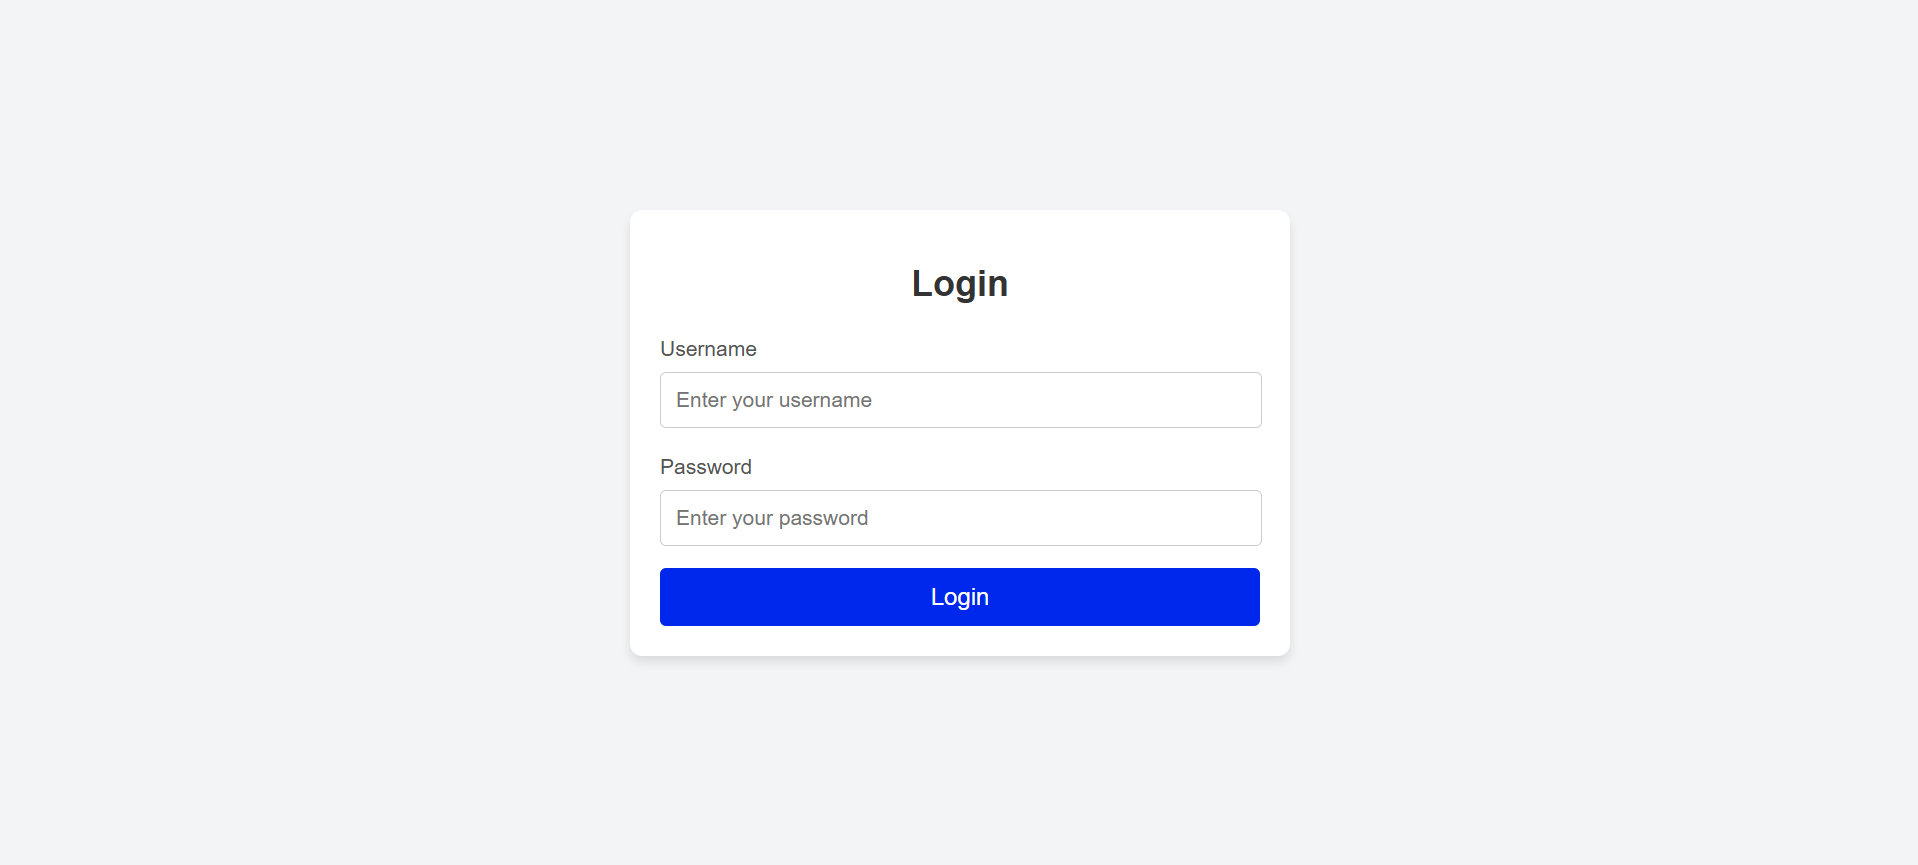
\includegraphics[width=0.6\linewidth]{login-full-size.png}
    \caption{Version 1 and 2, Full sized window}
    \label{v1-2-full}
\end{figure}

\begin{figure}[H]
    \centering
    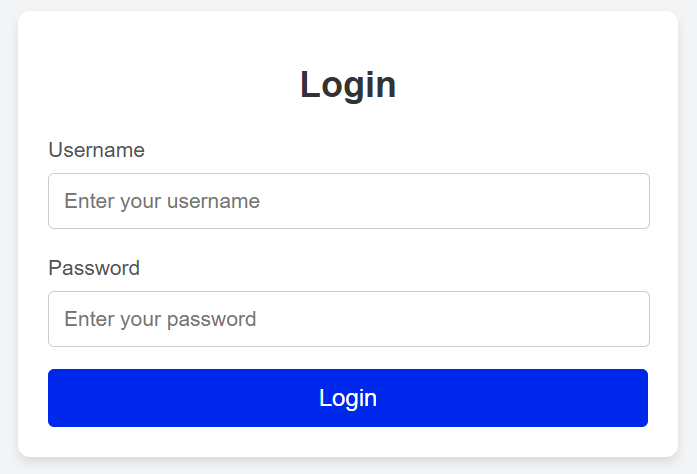
\includegraphics[width=0.6\linewidth]{login normal.png}
    \caption{Version 1 and 2 zoomed into login component}
    \label{v1-2-zoom}
\end{figure}

\begin{figure}[H]
    \centering
    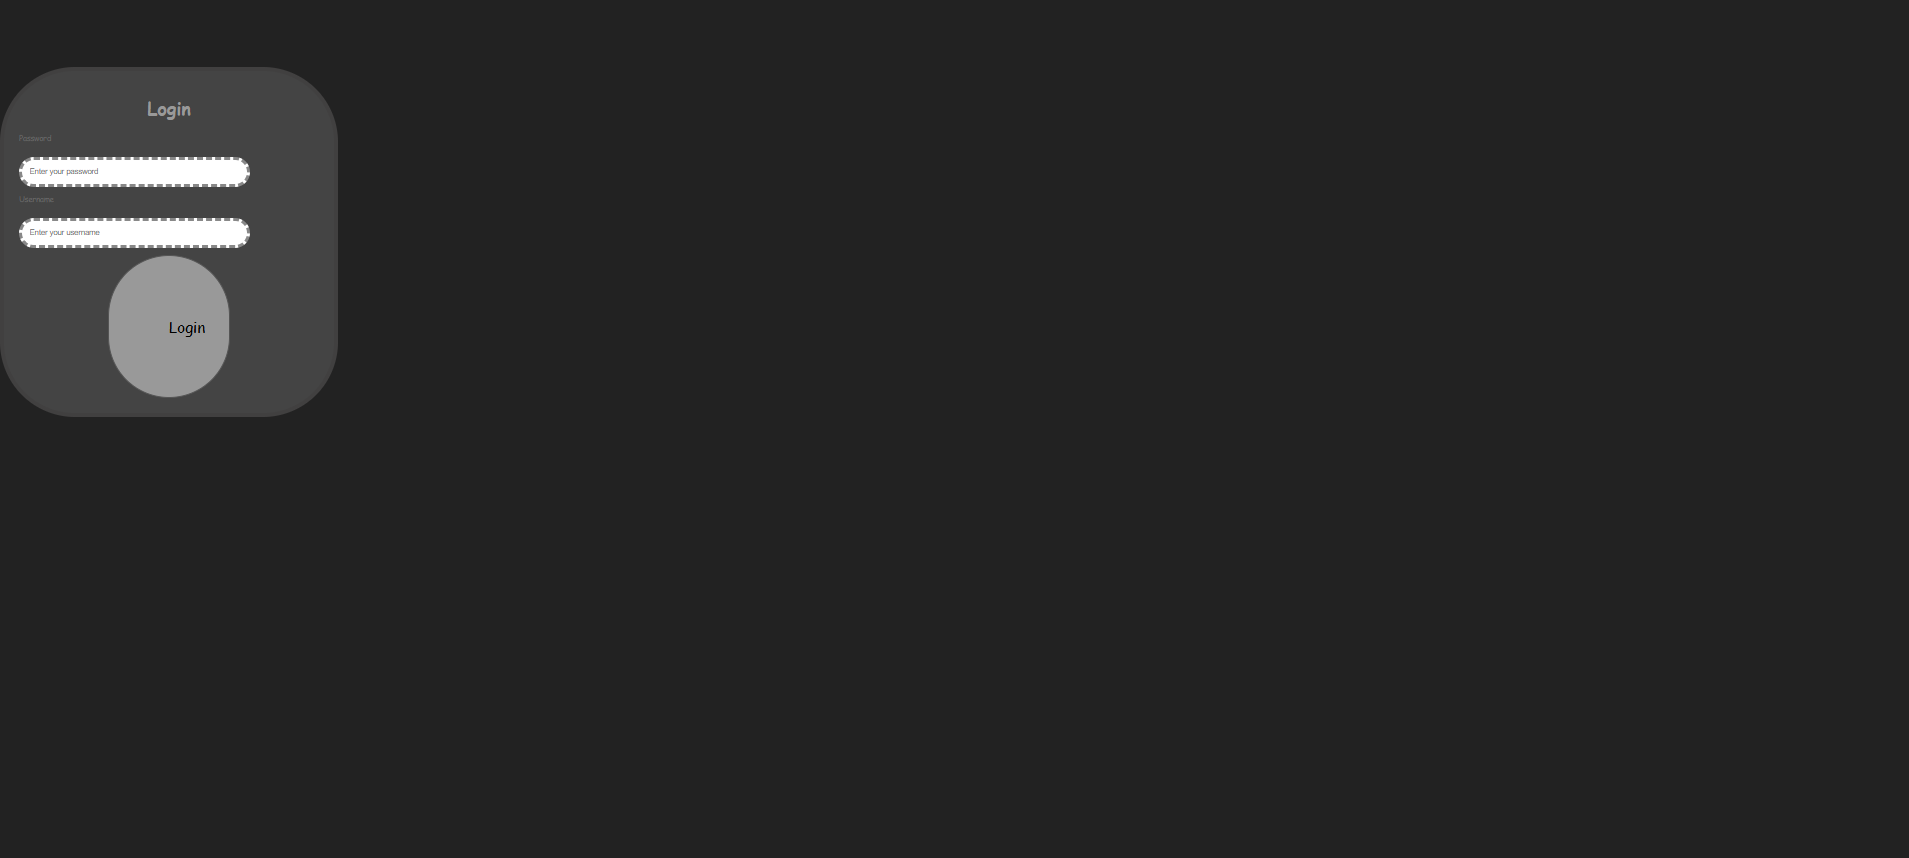
\includegraphics[width=0.6\linewidth]{V3 full size.png}
    \caption{Version 3 Full sized window}
    \label{v3-full}
\end{figure}

\begin{figure}[H]
    \centering
    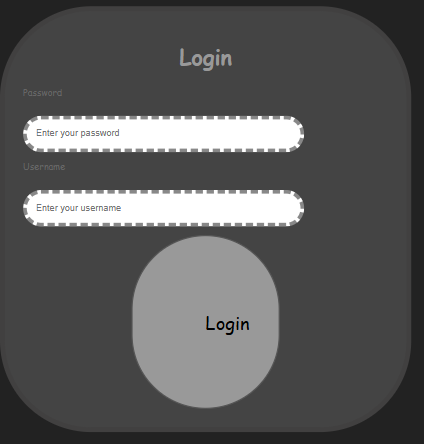
\includegraphics[width=0.6\linewidth]{V3 zoomed in.png}
    \caption{Version 3 zoomed into the login component}
    \label{v3-zoom}
\end{figure}

The produced website code is available in its entirety in appendix C.

\subsection{Checklist Development}
%A quality assurance checklist will be developed using sources like \href{https://www.softwaretestinghelp.com/login-page-test-cases/}{Software Testing Help}. The checklist will be categorized using the ISO/IEC 9126 software quality standards.
The quality assurance checklist was developed and categorized using the ISO/IEC 9126 software quality standards and their subcategories.

The checklist included the following criteria:

\textbf{Functionality}:
\begin{enumerate}[label=1.\arabic*]
    \item Verify that a user can log in with a valid username and valid password.
    \item Verify if a user cannot log in with a valid username and an invalid password.
    \item Verify that it says “Invalid username or password!” somewhere for invalid login.
    \item Verify if the data in password field is either visible as asterisk or bullet signs.
    \item Verify if the ‘Enter’ key of the keyboard is working correctly on the login page.
    \item Verify that the login button attempts a login.
    \item Verify that logging in will the take the user to /LoggedIn
    \item Verify that a user that is logged in to the correct account.
    \item Verify that the password is Case-sensitive
\end{enumerate}

\textbf{Reliability}:

\begin{enumerate}[label=2.\arabic*]
    \item Verify that it is possible to log in again after an error.
    \item Verify that logging in behaves the same way every time.
\end{enumerate}

\textbf{Usability}:

\begin{enumerate}[label=3.\arabic*]
    \item Verify that the font is easy to read.
    \item Verify that the contrast of text color and background has a high enough contrast
    \item Verify that the layout of the login page is as you would expect.
    \item Verify that the labels are useful.
    \item Verify that the page is not really ugly.
\end{enumerate}

\textbf{Efficiency}:

\begin{enumerate}[label=4.\arabic*]
    \item Verify the time taken to log in is less than 1 second.
    \item Verify that logging in is not unnecessarily complicated.
\end{enumerate}

\textbf{Portability}:
\begin{enumerate}[label=5.\arabic*]
    \item Verify that the login page works on Google Chrome.
    \item Verify that the login page works on Microsoft Edge.
    \item Verify that the login page works on Safari.
    \item Verify that the login page works on Firefox.
    \item Verify that the login page works on a smartphone.
\end{enumerate}

\subsection{Automated Testing Using Cypress}
Cypress was used to automate tests that evaluate the quality of the login page against the checklist criteria. The tests for \textit{functionality} mostly consisted of simulating writing the username and password and testing if the website behaves as expected.

The tests for \textit{reliability} related to the capability of software to maintain its level of performance over time. This includes recoverability, the ability to recover from errors and reliability compliance where the login page is expected to work the same every time. To test recoverability, tests were made to intentionally produce an error by typing the wrong password and then attempting to log in. Reliability compliance was tested by logging in 50 times.

Usability testing was automated by making assumptions about what it means to have an expected layout and a nice looking website. The assumptions were that an expected layout means that elements should come in the order of username, password and then button. A login website that is "not really ugly" was assumed to have readable text, an expected layout, centered elements and appropriate spacing between elements. The tests that made sure that the elements are centered on the screen also made sure that they were aligned with each other. Label usefulness was tested by making sure that the text above username says something close to "user" and the same for the label describing the password input field.

Efficiency testing was automated by measuring the time between starting a login attempt and the login screen appearing. In addition to the time it takes for the software to complete its task, tests were also written in a way that ensured that the login process was not too complicated for the user. This was done by ensuring that there were exactly two input fields. If there are more input fields one can assume that the login page is too complicated and time-consuming for the user. Furthermore, the tests ensured that there was exactly one field responsible for the username and exactly one responsible for the password.

Portability was tested by running all the tests again for all the different browsers in the specification.

\subsection{Hypothesis} Before testing began one hypothesis was that some issues, such as subjective usability concerns, would not be detectable by Cypress. Another hypothesis was that humans are error-prone in their nature and that this would hurt their consistency in finding errors across several people. The team were not sure which categories of issues would be hard for a human to test. If a user has a Windows computer testing Safari is exceedingly difficult, but it is not impossible. The research team had an idea that the test subjects would believe it impossible and not attempt to find a solution to this problem. The team had high confidence that the assumption that some issues can only be identified by humans and some can only be identified by a computer was true. We believed that the testing would result in an interesting Venn diagram outlining the overlap, intersection and difference of the sets of faults that can be identified by either method.

\subsection{Human Testing with Real Users}
\textbf{Participant Selection}: Four people participated in the testing in total. All test subjects study computer science or information and communication technique at LTH. One of the test subjects participates in the course that this research project is connected to; a course called 'Software Testing' at LTH.

\textbf{Testing Procedure}:
The finished website code was uploaded to a cloud service called Netlify so that the test subjects could display it on their own devices. The test subjects were given a paper with the scenario, a list of the valid login-information and the quality assurance checklist. The exact scenario given is available in appendix A. The participants were then asked to follow the checklist's criteria and evaluate if it was true for the given version of the website. The participants followed through with the checklist for each of the three versions, all the while ticking off what true, and circling what was false. If the test subject was unsure they left it blank.

\section{Results}
\subsection{Test Creation}
Using Cypress to create automated testing turned out to be mostly straightforward and not too complicated. There were a few hurdles that we had to overcome.

\begin{enumerate}
    \item Cypress does not support Safari. There is experimental support for Safari using the open source browser engine WebKit which Safari is built upon. This means that the tests are not run in the actual Safari browser. This could potentially lead to differences in how the website is displayed and how the tests are run.
          % DISCUSS, it turns out that WebKit has the same user agent as Safari when running tests in Cypress and they should have the same functionality since Safari is built on WebKit.
    \item The usability tests had a lot of complicated code to compare layout alignment, ordering and color contrast. Cypress does not natively support this kind of testing. Testing how long something takes or simulating pressing a key on the keyboard for example has native support which makes that kind of testing easy and efficient. Usability testing turned out to be possible but not easy.
          %% Discuss: Cypress does not have native support for this kind of testing because the assumption that we have, that Usability testing with automated programs is unneccessary if not impossible, is held by a lot of other people. 
\end{enumerate}

The test code is available in its entirety in the appendix B.

\subsection{Automated Testing Results}
The results from running the test have been compiled to 4 reports, one for each browser supported. The reports are available at appendix E.
After the test reports were compiled the team used them to determine the checklist validity. The research teams interpretation of the results are outlined in its entirety in appendix E.
In order to compare automated testing with human testing the results from both are compiled in a Google Sheets document available in appendix D.
The accuracy of the answers are outlined below.
\subsubsection{Fully functional}
All tests passed which lead the team to believe that all the requirements are fulfilled. This was also the correct answer according to the keys that the team had prepared before initiating testing.

\subsubsection{Mostly reliability and portability issues}
Checklist item 3.1 \textit{Verify that it is possible to login again after an error} was incorrectly marked as TRUE. In the testing code an error is produced by attempting to enter an incorrect password, but in this version every password is correct, so no error is produced. This issue would be remedied by creating a test that produces an error by entering an incorrect username as well.

\subsubsection{A lot of issues}
Surprisingly version 3 that we thought would be difficult for the automated testing suite to evaluate did not have any mistakes. The tests would suggest that the labels are useful because it says "Username" and "Password" on them. The tests show that the font is not a usual one and the font size is too small, and the contrast is bad and hard to read. The team made the call that the labels are not useful based on this information.

In summary all the issues that we set out to test \textit{can} be identified with automated testing.

\subsection{Human Testing Results}:
The results from the human testing was inconsistent, but all issues had at least one correct answer from one of the test subjects. The humans were terrible at identifying Portability issues because if they did not have the browser requested they did not make efforts to test it on a friends computer or install a new browser. Some test subjects assumed that it would work on the other browsers because they could not be bothered to test it out, or did not answer. Other test subjects mistakenly assumed that the site worked on a given browser because it loaded correctly. If they had attempted to log in they would find out that it does not work. The automated tests ran by the computer had no issue running all the tests again with a different browser. Boredom and laziness is not a factor for the computer. For version 3 one test subject could not log in because they did not try the admin account which gave wildly inaccurate results and tracking the biggest fault would be difficult. The computer did not have any issue logging in with each account.

\subsection{Analysis of Overlap and Differences}
Let A be a set of issues found by automated testing and B be a set of issues found by human testing. Using some set operations we can answer our research questions.
\subsubsection{Union $(A \cup B)$ Issues identified by either method.}

There are no type of issues that cannot be identified by either automated tests or human testers because automated tests {\textit{can}}{can} identify all types of issues we set out to find.
\subsubsection{Intersection $(A \cap B)$ Issues identified by both methods.}

Since at least one human correctly identified each issue. The overlap between the two methods is 100\%.

\subsubsection{Unique to either (A \textbackslash B) Issues only detected by automated testing.}

This is an empty set since all issues \textit{can} be identified by either methods.

\subsubsection{Unique to Human Testing (B \textbackslash A) Issues only identified by human testers.}

This is an empty set since all issues \textit{can} be identified by either methods.
\subsubsection{Union complement $(A \cup B)^c$ Issues not found.}
This is an empty set since all issues \textit{can} be identified by either method.

\subsection{WebKit vs Safari}
The testing team was worried that WebKit and Safari would not behave the same way during testing and would for example have different User Agents. According to the Mozilla Developer Network the HTTP User-Agent request header is a characteristic string that lets servers and network peers identify the application, operating system, vendor, and/or version of the requesting user agent. % HJÄLP HUR SKA JAG CITERA?? https://developer.mozilla.org/en-US/docs/Web/HTTP/Headers/User-Agent todo

To determine the user agent the testing team used the following code:

\begin{lstlisting}[caption=Detect Safari Browser, label=code:safari]
let isSafari = /^((?!chrome|android).)*safari/i.test(navigator.userAgent);
\end{lstlisting}

When asserting if this is true or not it was true in WebKit but false in Chrome, Firefox and Microsoft Edge. This signifies that the user agents are the same on WebKit and Safari. Playwright is the engine under the hood of the Cypress testing suite. According to the official Playwright documentation, running WebKit simulations on a Mac is very close to the real experience, but some issues arise if you run it on the most affordable option of a Linux system. For example video playback may not behave as expected. % https://playwright.dev/docs/browsers
This happened to not be an issue for the testing team since one of the team members have a MacBook and one of the team members have a Windows computer. Running WebKit with Playwright on a MacBook is stated to be as close to running on closest-to-Safari experience as possible according to the documentation.

\section{Discussion}
\subsection{Creative Feedback}
The results of the testing prove our hypothesis about the strengths and weaknesses of both automated and human testing to a strong degree. However, some new key insights were also found. The automated tests were more accurate in finding issues on the login page with no human finding all problems. The automated tests could not, in contrast to human testing, give any creative feedback. The user feedback obtained during the testing gave us new insights about our program that the team had not thought about in cases even altered the opinion of the team of what the correct answer to a problem was to begin with.

The human testing had a large variance in the problems found whereas the automated testing always gives the same results. The variance could be explained by many factors, since the test subjects are different from each other in very meaningful ways.

\subsection{Human Motivation}
The test subjects in general lacked motivation. Results from the portability testing show that people generally do not install a new web browser for test purposes. Nor did the test subjects try to use their friends' computer. Some test subjects did not care to test it even if they had the correct browser installed. Even the ambitious and motivated test subjects felt done after testing if the login worked at all, whereas the computer ran all the tests again on all the browsers without complaining. Most test subjects had low motivation, probably due to a lot of factors but most importantly the following:

\begin{enumerate}
    \item They do not get paid to do the work, but they do the testing out of their own good will.
    \item Most test subjects did not find satisfaction in repetitive tasks. A good test subject who enjoys the task might do better.
\end{enumerate}

We did not have the resources to spend more time in order to find test subjects that enjoy repetitive tasks. Additionally, we did not have the resources to pay the test subjects with anything else than gratitude. If we were to retry this experiment with more resources we attempt to fix both of those issues. The problem with putting too many resources to compensate for human weakness is that a computer does not have these problems. One could argue that makes the factor irrelevant. The computer will never question the importance of testing and will always try to do as they are told.


\subsection{Results vs Hypothesis}
The team honestly thought that there probably are some issues can only be
identified by humans and vice versa. Furthermore, the team believed that there were some issues that would not be identified by either method. This turns out to also be false. The Venn diagram that would be produced by the results that we found would not be interested in the slightest. All the types of issues can be identified by both methods, the diagram would be a mono colored block.   However, the computer definitely has the edge on most kinds of testing, but humans can exceed the expectations of the person writing the tests. This may be ratified as well using AI to ask for subjective opinions and suggestions. When asking popular AI chatbot ChatGPT whether the first/second version or third version looks better it responds like this: "The first image (version 1/2) is aesthetically more appealing according to modern design standards. It follows the principles of minimalist design with clear lines, good contrast, and readability. It uses a light background and a blue button to highlight the most important interaction (the login button), making it more user-friendly and professional.

The first image feels more playful but less modern and professional. The dark background and outlines can give an overwhelming impression, especially for users who prefer simplicity and clarity.

If the goal is to create a more user-friendly and modern experience, the second design is preferable.". This suggests that modern AI can be used to make reports on subjective issues.

\subsection{Exceeding Expectations}
Writing tests in Cypress will only be as good as the faults that the people writing the tests can imagine. The only real issue that the computer did not find was that in version 2 was the missing recoverability. When writing the tests the testing team assumed that writing the wrong password would produce an error. This shows that the accuracy and reliability of the test is limited by the knowledge, imagination and skill of the test writers. Using modern tools like ChatGPT the test writers can mitigate this factor somewhat, but we believe that no matter how good you are some things will inevitably be missed. One could however argue that this fault was irrelevant because if writing the wrong password does not produce an error recoverability is a minor issue until that is fixed. If the security issue were to be fixed then the tests would work as intended. Additionally, some humans made the same mistake because in version 2 there is a risk of random failure every time a login is attempted. This error is possible to recover from which confused the humans and made some of them think that every fault would behave the same. Some test subjects were initially confused when attempting to produce a fault since every password worked. After a short thinking period all test subjects came to the conclusion that they should try to change the username, Cypress can not deliberate and alter their testing methods based on unexpected results.

\subsection{Writing automated Usability tests}
Writing usability tests is much harder than the other kind of tests. The reason it was hard was because we had to write a lot of the logic ourselves. We believe the tools for this kind of testing is not included in most testing suites due to the commonly held belief that running usability tests with a computer is fruitless because only humans can do accurate testing. This turned out not to be true.

As it stands right now writing Usability tests seem to not be worth it due to the difficulty, but we believe that this is an issue with insufficient tooling and not a problem that is unsolvable.

\subsection{Recommendations}
With the existing tooling that is available today, using a combination of automated tests together with human user testing yields the most accurate test results. The automated tests have greater accuracy and are easier to perform, and testing with humans gives more depth and could help make the tests more effective with creative feedback.

\subsection{Limitations of the project}
The login website is a quite small website with only one functionality, to log in. This creates a testing scenario with a very small scope, and the functionality is isolated. In more common websites, a login page would be a small part of the website and would need to be integrated with the rest of the application. This means the testing was a bit simpler, and might not be able to show how human testing compares to computer testing on a larger scale when it comes to efficiency. The testing can however show patterns in what type of criteria human testers or computers, lack in or excel at testing. We picked a login page because of these main reasons.

\begin{enumerate}
    \item It's very common on the web, which means that all users have preexisting conceptions of how it should work.
    \item It's not too complicated to make.
    \item It's very important that it works as the user would expect, and that it works well, or the user will not be able to even try the product or service. We believe that if the login page does not work all other type of testing is irrelevant making it the most important part of a web-based business
\end{enumerate}

\section{Conclusion}
\subsection{Summary}
In conclusion, automated tests proved more robust and highly reliable, additionally Cypress was able to find the intended design errors; something that was unexpected. The human testers provided inaccurate and inconsistent results as well. The automated testing did not give feedback directly on the tests or application itself, and human testers gave significant details that previously were not realized. We have found that human testing might provide something that an automated test cannot but in that case it is something that we did not look for. Finding this out would require further research.

\section{Future Work}
\subsection{Is human creativity unique?}
We have found something that humans were better than our tests at that we did not expect to find. Is this unique to humans or is it possible to do the same with AI? Early research like the ChatGPT example from earlier suggest that it is not unique to humans. We recommend further research to answer the question "To what degree can human creativity in giving feedback in user testing be reproduced by automated Black-Box testing?". Our hypothesis is that most if not all the human strengths are not unique to humans. Creating a testing suite that gives this kind of feedback would be a valuable tool. One could very easily use Cypress to automate this process. Here is a suggestion to how this could be done:

\begin{enumerate}
    \item Take a screenshot with Cypress
    \item Send the screenshot to an AI, and ask if it is visually appealing TRUE or FALSE
    \item Assert that the answer is TRUE.
\end{enumerate}

This might make it possible to test subjective opinions with Cypress. By sending screenshots with each interaction you may get good spontaneous and unexpected feedback from the AI as well. It would be interesting to see if the AI generally gives better feedback than humans, and if it would be cheaper to run automated tests even when compensating for the cost of the test developer and the cost of using an AI. The AI requirements are quite resource intensive, the most costly is the image recognition and sending images to the AI. Our hypothesis is that AI would give better and more consistent feedback than humans and that this method could potentially entirely replace human testing the unit, integration and system level. Acceptance testing will always have to be done by a human because testing in theory and on a real phone can be very different. Another hypothesis is that the feelings that users get when using a product can not be accurately simulated and estimated by an AI.

\subsection{Can a website be ugly and useful?}
Our findings suggest that there is a tight link between beauty and usefulness. Is there such a thing as an ugly website that is easy to use? Would it be generally easier to use if it was more pretty? Would it be more pretty if it was easier to use? Our hypothesis is that they are strongly linked, but an interface that is ugly can still be easy to use, but making it easier to use would also make it prettier at the same time.

\subsection{Is Playwright + WebKit an accurate representation of Safari?}
We found that Playwright and WebKit was very similar to Safari, but there are things that probably behave differently. Would it be possible to create a test case in Cypress that fails on Playwright + WebKit but would succeed with Safari? The main difficulty with this further research is that you cannot use Cypress with Safari which is the entire reason why we used WebKit to begin with. One would have to either use some other suite that might have Safari support, or do the testing manually.

\subsection{Including maintainability}
Maintainability was excluded from the research because we wanted to specifically focus on Black-Box testing. Evaluating whether humans or computers are better at evaluating maintainability would require White-Box testing methods.

\subsection{Evaluate effectiveness}
This project only tried to find if it was possible at all to identify categories of issues. The results suggest that it would be more research is required to determine the degree to which humans are better at one kind of testing compared to another since it turns out that all categories can be identified by either method.

\section{Contribution statement}

Oliver: Project planning, report writing, produce the checklist, compiling the results from the user testing, produce automated tests, run the user tests, interpret the test results, publish the website to the cloud, prepare the scenario, run the tests and compile reports from the results.

Kristina: Project planning, report writing, produce the checklist, compiling the results from the user testing, produce the website code, run the user tests.

Adam: Project planning, report writing, produce the checklist, produce automated tests.

Emma: Project planning, report writing, making the checklist, compiling the results from the user testing, produce the website code, interpret the test results.


\begin{thebibliography}{9}
    \bibitem{ISO} ISO/IEC 9126, Software engineering — Product quality, The International Organization for Standardization, 2001-06.
\end{thebibliography}

\appendices
To save space all of the appendices are links. All links have corresponding QR codes.
\section{Scenario}
The user scenario that was presented to the human test subjects:
\href{https://bit.ly/scenario-user-testing}{https://bit.ly/scenario-user-testing}
\begin{figure}[h!]
    \centering
    \includegraphics[width=0.25\linewidth]{qr-codes/scenario.png}
    \caption{Appendix A: Scenario}
    \label{fig:enter-label}
\end{figure}

\section{Cypress Test Code}
The test code that was run to produce the automated test results.
\href{https://bit.ly/cypress-code}{https://bit.ly/cypress-code}

\begin{figure}[H]
    \centering
    \includegraphics[width=0.25\linewidth]{qr-codes/cypress-test-code.png}
    \caption{Appendix B}
\end{figure}

\section{Github Repository}
The GitHub Repository in its entirety which includes the code for the different versions of the login page.
\href{https://bit.ly/complete-repo}{https://bit.ly/complete-repo}

\begin{figure}[H]
    \centering
    \includegraphics[width=0.25\linewidth]{qr-codes/github-repo.png}
    \caption{Appendix C}
\end{figure}


\section{Results comparison}
A Google Sheets document comparing our key, the computers answer and the degree to which all human test subjects answered correctly for each version.
\href{https://bit.ly/results-comparison}{https://bit.ly/results-comparison}
\begin{figure}[h!]
    \centering
    \includegraphics[width=0.25\linewidth]{qr-codes/results-comparison.png}
    \caption{QR code to the appendix D}
\end{figure}

\section{Automated test reports}
The test reports that were generated after running the automated tests.
\href{https://bit.ly/results-automatic}{https://bit.ly/results-automatic}

\begin{figure}[H]
    \centering
    \includegraphics[width=0.25\linewidth]{qr-codes/results-automatic.png}
    \caption{Appendix E}
\end{figure}


\end{document}
